\documentclass[10pt,twocolumn,letterpaper]{article}

\usepackage{cvpr}
% Figures live in the Part 1 directory in the repository.
% In Overleaf, upload the figure PDFs alongside main.tex.
\graphicspath{{../Part 1/}}


\definecolor{cvprblue}{rgb}{0.21,0.49,0.74}
\usepackage[pagebackref,breaklinks,colorlinks,allcolors=cvprblue]{hyperref}
\def\paperID{*****}
\def\confName{CVPR}
\def\confYear{2026}

\title{Predicting Clinical-Trial Stopping Reasons and Outcomes\\[0.4em]
{\normalsize\normalfont CS5785 / ORIE5750 / ECE5414 Midterm Project}}

\author{Davide Bacchini\\{\small Part 1 models and figures}
\and Aakarsh Gundu\\{\small Part 1 challenger and Part 2 evaluation}
\and Priyansh Raval\\{\small Part 2 models and error analysis}}

\begin{document}
\maketitle

\begin{abstract}
We study clinical trials from the HINT benchmark in two steps.
First we predict why trials stopped early (Safety, Funding, Efficacy, Recruitment and Other) when only 157 of 1{,}171 training trials have labels.
We compare clustering, label spreading and self-training. We combine logistic regression and a linear SVM with evidence from nearby labeled trials and choose the reason set with the highest expected F1. The best submission reaches a public sample F1 of 0.89871, against 0.871 for the course baseline.
We then predict trial success in each phase. A blend of pooled TF--IDF logistic regression and cosine nearest neighbors reaches public log loss of 0.59100. It lowers the fraction of failed validation trials predicted successful in all three phases. The largest drop is in Phase~I, from 46.9\% to 40.6\%.
\end{abstract}

\section{Methods}
The project has two tasks on clinical trials from the HINT benchmark~\cite{fu2022hint}.
We first predict the stopping reasons of the trials and then whether each trial is successful.
For the stopping reasons we have 1{,}171 training trials but only 157 of them have labels.
These are the earliest 10\% of the trials plus 40 trials picked to include more of the rare reasons, so they are much older than the test trials, which start between 2010 and 2016.
Each trial is described by a 150-dimensional embedding of its stopping-reason text, which was made with a sentence-embedding model, reduced with PCA and randomly rotated.
We also use the start year, scaled with the mean and standard deviation of the training trials.
All models are trained with scikit-learn~\cite{pedregosa2011scikit}.

\begin{table*}[!t]
\centering
\footnotesize
\setlength{\tabcolsep}{4.75pt}
\begin{tabular}{lccccccccc}
\hline
 & \multicolumn{7}{c}{Val} & Older to & Kaggle \\
Model & Sample F1 & Macro F1 & Safety & Funding & Efficacy & Recruit. & Other & newer & public \\
\hline
LR, labeled trials only & 0.868 & 0.719 & 0.941 & 0.400 & 0.720 & 0.961 & 0.571 & -- & -- \\
k-means labels directly & 0.744 & 0.444 & 0.424 & 0.000 & 0.444 & 0.970 & 0.381 & -- & -- \\
GMM labels directly & 0.709 & 0.465 & 0.588 & 0.000 & 0.417 & 0.891 & 0.429 & -- & -- \\
Label spreading directly (30 neighbors) & 0.833 & 0.536 & 0.700 & 0.000 & 0.667 & 0.980 & 0.333 & -- & -- \\
LR + k-means pseudo-labels (weight 0.05) & 0.793 & 0.586 & 0.581 & 0.400 & 0.600 & 0.970 & 0.381 & -- & -- \\
LR + confident label spreading labels & 0.863 & 0.687 & 0.900 & 0.400 & 0.720 & 0.970 & 0.444 & -- & -- \\
LR + confident GMM labels & 0.880 & 0.720 & 0.947 & 0.400 & 0.636 & 0.980 & 0.636 & -- & -- \\
KNN cosine ($k=5$), labeled trials only & 0.868 & 0.614 & 0.750 & 0.000 & 0.815 & 0.980 & 0.526 & -- & -- \\
LR + start year, labeled trials only & 0.876 & 0.738 & 0.941 & 0.400 & 0.750 & 0.961 & 0.636 & -- & -- \\
LR + start year, self-training 1 round & \textbf{0.902} & \textbf{0.810} & 0.941 & 0.667 & 0.846 & 0.961 & 0.636 & -- & 0.874 \\
LR + start year, self-training 2 rounds & 0.893 & 0.746 & 0.941 & 0.400 & 0.846 & 0.970 & 0.571 & 0.821 & 0.875 \\
\quad + best expected F1 & 0.893 & 0.746 & 0.941 & 0.400 & 0.846 & 0.970 & 0.571 & 0.823 & 0.884 \\
SVM unit length, self-training 2 rounds + best F1 & 0.878 & 0.765 & 0.900 & 0.667 & 0.769 & 0.935 & 0.556 & \textbf{0.857} & 0.886 \\
Average of LR and SVM + best F1 & 0.887 & 0.780 & 0.947 & 0.667 & 0.769 & 0.971 & 0.545 & 0.851 & 0.892 \\
LR/SVM + joint reason sets and neighbors & 0.897 & 0.798 & 0.947 & 0.667 & 0.815 & 0.952 & 0.609 & -- & \textbf{0.899} \\
\hline
\end{tabular}
\caption{Reason models. Validation fits use 157 observed labels and, where applicable, the unlabeled training pool. Older to newer is the sample F1 on the newer trials averaged over the cut years 2002--2006. Kaggle is the public leaderboard, where the course baseline scores 0.871.}
\label{tab:reasons}
\end{table*}

\paragraph{Semi-supervised labeling.}
Since most training trials have no labels, we compare four methods to label the other 1{,}014.
The first one is k-means clustering on all training trials.
We first reduce the standardized embeddings to 20 principal components, which keep about 70\% of the variance.
Then we run k-means with $k=10$ and 10 restarts, starting from a k-means++ initialization.
Each cluster gets the reasons that at least half of its labeled trials have and every unlabeled trial takes the reasons of its cluster.
The second one is a Gaussian mixture model (GMM) on the same 20 components, with diagonal covariance and $k=20$ chosen by BIC~\cite{schwarz1978estimating}.
Unlike k-means, every trial gets a probability for each cluster, so the reason probabilities of a trial are the reason shares of the clusters weighted by these probabilities.
The third one is label spreading~\cite{zhou2004learning} on a kNN graph, run separately for each reason.
We use 30 neighbors, which worked better than 10 and 20, with $\alpha=0.2$ and at most 100 iterations.
Some trials are not connected to any labeled trial, mostly because many trials have exactly the same embedding.
In fact there are only 859 different embeddings among the 1{,}171 training trials.
For these trials we use the share of each reason in the labeled data as their probabilities.
We test downweighting the labels from k-means and label spreading. For GMM and label spreading, we also test keeping only confident labels.
The fourth method is self-training, where a classifier trained on the real labels predicts the unlabeled trials.
We keep only the trials where the classifier is sure about all five reasons, with a probability above 0.8 or below 0.2.
Then we train again on the real labels plus these predicted labels, repeating this for two rounds.
Each round starts again from the real labels, so wrong predictions from the first round do not stay in.

\paragraph{Models and features.}
We compare three classifiers, starting with a logistic regression for each reason with $C=10$. The second is KNN with $k$ from 3 to 15, using either Euclidean or cosine distance and we also try averaging it with the logistic regression. The third is a linear SVM for each reason with $C=0.1$, which gives probabilities through Platt scaling~\cite{platt1999probabilistic}.
As features we compare the standardized embeddings, the start year, Morgan fingerprints of the matched drugs (1{,}024 bits, maximum over the drugs of a trial and all zeros when no drug is matched) and everything together.
Since the embeddings were randomly rotated, individual columns have no direct interpretation.
For this reason we also try scaling each embedding to length 1 instead of standardizing the columns.
Our initial ensemble averages self-trained logistic regression on standardized embeddings plus start year and a self-trained SVM on unit-length embeddings.

\paragraph{Decision rule.}
The simplest rule gives a trial every reason with a probability of at least 0.5, or only the most likely one if none reaches 0.5.
We also tried a different threshold for each reason, tuned on val.
Since Kaggle scores sample F1, in the end we choose for each trial the set of reasons with the highest expected F1~\cite{ye2012optimizing,dembczynski2011exact}.
We go through all 31 nonempty reason sets and choose the one with the highest expected F1. The initial ensemble assumes independent reasons when forming set probabilities. The final blend puts 25\% weight on a classifier for whole reason sets, trained with approximate RBF features and two rounds of downweighted self-training. We also blend in the reason sets of eight nearby labeled trials, giving them more weight for close cosine matches.

\paragraph{Model selection.}
The val trials come from the same years as the training trials, but all test trials are from 2010 to 2016.
To see how each model does on newer trials, we train it on the 235 trials with real labels that started up to a cut year and test it on the ones that started later.
We repeat this for every cut year from 2002 to 2006 and report the average of the five scores.
We compare the models on both val and this average and when they disagree we trust the newer trials more, since they are closer to the test set.
The final submission refits with all 235 observed labels and the unlabeled training pool.

\paragraph{Outcome models.}
For each trial-phase row we predict whether the trial met its primary endpoint. We use 8{,}037 training rows and 1{,}013 validation rows. We concatenate eligibility criteria, diseases, drug names and ICD codes. We compare a phase success-rate baseline, binary bag-of-words logistic regression, multinomial naive Bayes, cosine KNN, and logistic regression with unigram or unigram--bigram TF--IDF. The original classifier fits a separate TF--IDF logistic regression in each phase ($C=3$). To share information across phases, we then fit one logistic regression with phase indicators. We test a start-year feature, a matched-drug flag and Morgan fingerprints. The final ensemble averages the pooled model ($C=3$) with the drug flag at weight 0.7 and a separate distance-weighted cosine KNN ($k=30$) in each phase at weight 0.3. We select settings using validation log loss and a calendar check that fits on training trials through 2010 and evaluates on 2011--2013.

\paragraph{Outcome errors and calibration.}
We use 0.5 for binary predictions and report F1, ROC-AUC, average precision (AP), and log loss. We match unsuccessful validation trials to the reason labels saved by the initial Part~1 LR/SVM ensemble by trial ID. A failure can contribute to several reasons in its phase, and unmatched trials form their own group. Stopping reasons enter only the error analysis. We test sigmoid and isotonic calibration of the final blend with predictions from three training folds grouped by trial ID. We fit a separate map for each phase. The Kaggle submission uses the raw blend, refit on the combined training and validation rows after model selection, with probabilities clipped to $[0.001,0.999]$.

\section{Results}

Table~\ref{tab:reasons} shows the reason models on val, together with the older-to-newer score and the public Kaggle score for the versions we submitted.
Direct k-means, GMM and label spreading give sample F1 of 0.744, 0.709 and 0.833, below 0.868 for logistic regression on the 157 labeled trials. Adding confident GMM labels raises sample F1 to 0.880. Self-training gives the strongest validation improvement, reaching 0.902 sample F1 and 0.810 macro F1.
The SVM on unit-length embeddings scores lower on val, 0.878 against 0.893, but higher on the newer trials, 0.857 against 0.823.
Averaging the two models gives 0.892 on Kaggle, against 0.871 for the course baseline. The joint-set and neighbor blend changes 16 test predictions and raises public F1 to 0.89871. On validation it raises sample F1 from 0.887 to 0.897. Across four calendar cutoffs its mean is 0.875 versus 0.877 for the initial ensemble. On the latest holdout, 2008--2010, it raises sample F1 from 0.901 to 0.914.
Choosing the set of reasons with the best expected F1 changes only 6 of the 312 test predictions but adds almost 0.01 on Kaggle.


\paragraph{Outcome prediction.}
The phase-rate baseline and starter bag-of-words model have mean validation log losses of 0.672 and 0.940. Regularized TF--IDF improves that to 0.568. Table~\ref{tab:outcomes} shows that the blend further lowers log loss and raises ROC-AUC and AP in every phase. Phase~I F1 drops as recall falls from 0.835 to 0.788. The selected blend reaches 0.59100 on the public leaderboard. Two train-only submissions from the separate experiments notebook scored 0.61463 for a recency-weighted logistic regression and 0.59458 for a blend with a text model and boosted trees. These submissions also differ from the selected blend in their final fit data.

\begin{table}[!t]
\centering
\footnotesize
\setlength{\tabcolsep}{2.25pt}
\begin{tabular}{lcccccccc}
\toprule
 & \multicolumn{2}{c}{F1} & \multicolumn{2}{c}{ROC-AUC} &
 \multicolumn{2}{c}{AP} & \multicolumn{2}{c}{Log loss} \\
Phase & Orig. & Blend & Orig. & Blend & Orig. & Blend & Orig. & Blend \\
\midrule
I & 0.763 & 0.753 & 0.780 & 0.790 & 0.824 & 0.840 & 0.569 & 0.556 \\
II & 0.614 & 0.655 & 0.724 & 0.744 & 0.714 & 0.725 & 0.606 & 0.592 \\
III & 0.812 & 0.835 & 0.775 & 0.798 & 0.872 & 0.881 & 0.529 & 0.506 \\
All & 0.727 & 0.752 & 0.765 & 0.784 & 0.806 & 0.820 & 0.568 & 0.551 \\
\bottomrule
\end{tabular}
\caption{Outcome metrics on the same validation rows. The all-row F1, ROC-AUC and AP are pooled across rows. The all-row log loss is the equal-weight average of the phase losses.}
\label{tab:outcomes}
\end{table}

\begin{table*}[!t]
\centering
\footnotesize
\setlength{\tabcolsep}{5pt}
\begin{tabular}{lrrrrrrrrrrrr}
\toprule
 & \multicolumn{4}{c}{Phase I} & \multicolumn{4}{c}{Phase II} & \multicolumn{4}{c}{Phase III} \\
Reason & $n$ & True & Orig. & Blend & $n$ & True & Orig. & Blend & $n$ & True & Orig. & Blend \\
\midrule
Safety & 8 & 1 & 37.5 & 50.0 & 13 & 1 & 46.2 & 30.8 & 8 & 1 & 50.0 & 50.0 \\
Funding & 4 & 1 & 50.0 & 50.0 & 4 & 1 & 25.0 & 0.0 & 0 & 0 & -- & -- \\
Efficacy & 2 & 0 & 100.0 & 50.0 & 10 & 0 & 30.0 & 30.0 & 8 & 0 & 87.5 & 75.0 \\
Recruitment & 23 & 2 & 39.1 & 30.4 & 89 & 12 & 22.5 & 20.2 & 22 & 5 & 63.6 & 63.6 \\
Other & 4 & 0 & 50.0 & 50.0 & 21 & 3 & 38.1 & 38.1 & 11 & 2 & 72.7 & 63.6 \\
No recorded reason & 28 & 0 & 53.6 & 46.4 & 144 & 0 & 34.7 & 34.7 & 82 & 0 & 57.3 & 56.1 \\
All failed & 64 & 4 & 46.9 & 40.6 & 265 & 16 & 30.9 & 28.7 & 123 & 7 & 59.3 & 57.7 \\
\bottomrule
\end{tabular}
\caption{False-positive rates in percent among failed validation trials. True is the number with an observed stopping reason. For the five recorded reason groups, the other labels are Part~1 predictions. A dash denotes an empty group. The all-failed row counts each trial once per phase.}
\label{tab:outcome-errors}
\end{table*}

\paragraph{Outcome errors by reason.}
Of 452 failed validation rows, 254 have no Part~1 record, 171 have a predicted reason, and 27 have an observed reason. Table~\ref{tab:outcome-errors} shows that the blend lowers the overall false-positive rate in all phases. For example, Phase~I Recruitment falls from 9 of 23 to 7 of 23, while Phase~II Safety falls from 6 of 13 to 4 of 13. Phase~I Safety rises from 3 of 8 to 4 of 8.

\section{Discussion}

\begin{figure}[t]
\centering
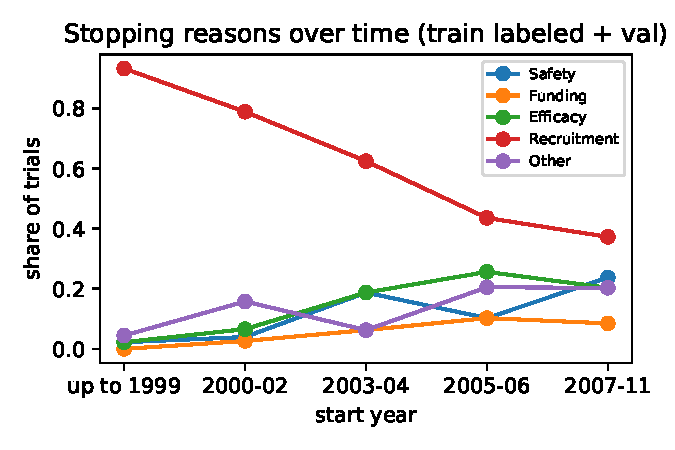
\includegraphics[width=\linewidth]{reason_share_by_year.pdf}
\caption{Share of each stopping reason among the 235 trials with real labels, grouped by start year.}
\label{fig:shift}
\end{figure}

\paragraph{Time and model selection.}
Figure~\ref{fig:shift} shows that the reasons for stopping a trial change a lot over time.
Recruitment goes from 93\% of the trials that started before 2000 to 37\% of those that started between 2007 and 2011, while Safety goes from 2\% to 24\%.
Since most labeled trials are old, a model trained on them predicts too much Recruitment for newer trials, and the test trials are the newest of all.
Adding the start year as a feature partly corrects this and raises sample F1 on val from 0.868 to 0.876.
For the same reason val can be misleading, since its trials come from the same years as the training trials.
On val the best model is self-training with one round at 0.902, while on the newer trials the SVM on unit-length embeddings is clearly better than the logistic regression, at 0.857 against 0.821.
The calendar check helped us choose the initial ensemble. The final joint-set blend improved public F1 and the latest calendar check, with a small decrease in the average over its four cutoffs.

\paragraph{Comparing the labeling methods.}
The k-means clusters often group together trials stopped for different reasons, as in one cluster where half of the labeled trials are Safety and half are Other, so all its trials get both reasons.
Funding is never the majority in any cluster, so no unlabeled trial gets it at all.
Label spreading instead struggles with the many trials that share exactly the same embedding.
These trials form small groups that are not connected to any labeled trial, and Funding ends up with an F1 of 0.
Adding the k-means and label-spreading labels makes logistic regression worse even with downweighting. Filtering the GMM labels helps, though the direct GMM labels miss Funding and often group several reasons together.
Self-training instead keeps only the trials where the classifier is already sure about all five reasons, so its predicted labels follow the same decision boundary and are mostly correct, and it still keeps some Funding trials.

\paragraph{Comparing the features.}
Adding the drug fingerprints to the embeddings lowers sample F1 from 0.868 to 0.842 and macro F1 from 0.719 to 0.608, and using everything gives the same result.
The embeddings capture the stopping text directly. The fingerprints add 1{,}024 sparse columns for 157 labeled trials, and 38\% of those trials have no matched drug.
Scaling the embeddings to length 1 helps the SVM a lot on the older-to-newer check (0.790 to 0.851) but not the logistic regression (0.807 to 0.804).
On unit-length vectors, distance depends on the angle between embeddings. That geometry appears to help the SVM more than logistic regression.

\paragraph{Comparing the decision rules.}
Tuning a threshold for each reason on val only moved Recruitment from 0.5 to 0.55 and changed val F1 by less than 0.01, which is about one trial out of 78, so we kept 0.5.
Choosing the set with the best expected F1 instead changes the prediction only when the classifier is unsure between reasons.
For example, if Other has probability 0.85 and Safety 0.48, predicting both loses little when Safety is wrong and gains a lot when it is right.
This changed only 6 test predictions but improved the public score from 0.875 to 0.884.
Validation has 78 trials and the public leaderboard uses about half of the 312 test trials. A few changed predictions can move either score.


\paragraph{Outcome errors and time shift.}
The original model has the highest false-positive rate in Phase~III, which also has the highest training success rate. Sharing word coefficients across phases can help Phase~I, which has only 1{,}012 training rows. Nearest neighbors add a different signal from similar trials. Drug fingerprints gave mixed results and adding start year did not improve official validation. Differences by reason are often just one or two trials. The true-label subsets contain at most 12 rows per phase and reason, so the predicted labels and small groups limit the comparisons.

Test trials in the supplied file start in 2014--2021, while training and validation end in 2013. In the calendar check, the improved model has a mean ROC-AUC of 0.724, down from 0.777 on official validation. Its mean log loss is 0.532, versus 0.554 for the original on the same calendar rows and 0.551 for the blend on official validation. A higher success rate on the newer rows (0.678 versus 0.536 in the earlier training cohort) can help explain why log loss improves while ranking gets worse. Public test log loss is higher still at 0.59100.

Sigmoid and isotonic calibration slightly lower official validation loss (0.5506 and 0.5491 versus 0.5511). On newer trials, both raise loss (0.5321 and 0.5419 versus 0.5317). We retain the raw blend.

\section*{Use of AI tools}
Aakarsh used OpenAI Codex to help implement and check model experiments, verify outputs, and edit the report.

{
    \small
    \bibliographystyle{unsrtnat}
    \bibliography{main}
}

\end{document}
